\documentclass[6pt]{AiTex}




\title{Memoria activad opcional}
\author{A.L.K.}
\date{Diciembre 2022}

\begin{document}
%\datos{facultad}{universidad}{grado}{asignatura}{subtitulo}{autor}{curso}
\datos{Informática}{Universidad Complutense de Madrid}{Ingeniería informática}{Métodos Algorítmicos en Resolución de Problemas}{Algoritmo de Prim y montículo de Williams}{Alejandro Barrachina Argudo}{2022-2023}
% \portadaApuntes
% \pagestyle{empty}
% \tableofcontents
% \pagestyle{empty}
\justify


\section*{Introducción}

En este documento se presenta la explicación de la practica opcional de MAR1, apartado 8, realizada por \autor.

\begin{multicols}{2}

    \chapterA{Algoritmo de Prim}
\section{Estructura de archivos}
La carpeta está estructurada de la siguiente manera:
\begin{itemize}
    \item\textbf{bin:} Carpeta que contiene el archivo final de compilación.
    \item\textbf{graph:} Carpeta que contiene los archivos de la biblioteca de grafos y casos de prueba:
    \begin{itemize}
       \item\textbf{graph.h y graph.cpp:} archivos con el código de implementación de grafos mediante listas de adyacencia y el propio algoritmo de Prim.
       \item\textbf{dummygraphs.h:} cabecera que introduce los grafos al programa.
       \item\textbf{test:} carpeta que contiene un generador de grafos aleatorio y los casos de prueba generados
    \end{itemize}
    \item\textbf{obj:} carpeta para la compilación de la librería de grafos.
    \item\textbf{main.cpp}: archivo fuente que corre los casos de prueba.
    \item\textbf{makefile}: archivo make para facilitar la compilación de la práctica.
\end{itemize}

\section{Pruebas}
Todas las pruebas incluyen los tiempos de carga desde archivo de los grafos y la salida por consola del arbol final. Todas las pruebas se realizan en el siguiente sistema:
\begin{itemize}
    \item\textbf{CPU:} i7-8750
    \item\textbf{GPU:} Nvidia Geforce GTX 1060 Mobile
    \item\textbf{RAM:} 16 Gb
    \item\textbf{SO:} ArcoLinux
\end{itemize}



Los gráficos de las pruebas se pueden ver en la figura \ref{fig:prim-plot}~(\nameref{fig:prim-plot})

\begin{figure}[H]
      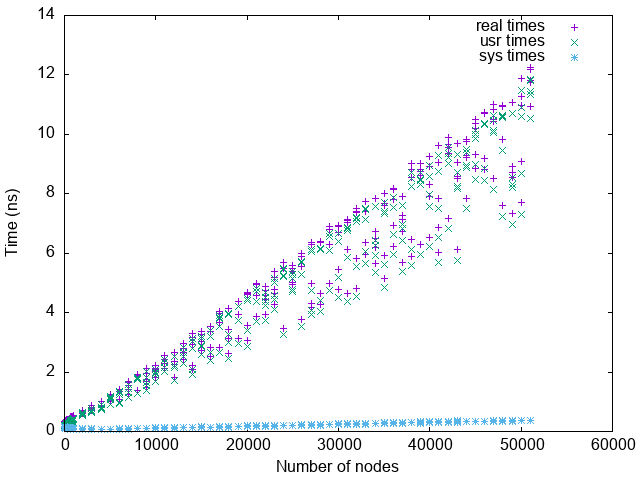
\includegraphics[width = \textwidth]{./images/prim-plot.png}
      \caption{Gráfica de tiempo del algoritmo de Prim para distintas cargas de trabajo.}
      \label{fig:prim-plot}
  \end{figure}


Los tiempos observados se pueden asimilar a las de una función $nlog(n)$, que es lo que se pedría en el enunciado.
A mayor numero de aristas en el grafo, mayor será el coste, pero en el algoritmo implementado si no hay unión (representado por el valor más alto de un int de 32 bits), no se hace ninguna operación y se pasa al siguiente nodo.

    \vfill
    \hfill

    \section{Montículo de Williams con Decrecer clave}
 {\small
  \subsection{Estructura de archivos}
  La carpeta está estructurada de la siguiente manera:
  \begin{itemize}
      \item\textbf{bin:} Carpeta que contiene el archivo final de compilación.
      \item\textbf{williams-heap:} Carpeta que contiene los archivos de la biblioteca de montículos y casos de prueba:
      \begin{itemize}
          \item\textbf{williams-heap.h y williams-heap.cpp:} archivos con el código de implementación de montículos mediante listas de adyacencia y el propio algoritmo de Prim.
          \item\textbf{dummyheaps.h:} cabecera que introduce los montículos al programa.
          \item\textbf{test:} carpeta que contiene un generador de montículos aleatorio y los casos de prueba generados
      \end{itemize}
      \item\textbf{obj:} carpeta para la compilación de la librería de montículos.
      \item\textbf{main.cpp}: archivo fuente que corre los casos de prueba.
      \item\textbf{makefile}: archivo make para facilitar la compilación de la práctica.
  \end{itemize}

  La implementación del montículo usada es la vista en los apuntes de clase, traduciendo los métodos de Daphny a C++.


  Los gráficos de las pruebas se pueden ver en la figura \ref{fig:decrease-key-plot}~(\nameref{fig:decrease-key-plot}). Estas pruebas incluyen la carga de un grafo desde fichero con todo lo que ello conlleva, pero no la generación del grafo como tal.

  Los tiempos observados se pueden asimilar a las de una función $log(n)$, siendo n el número de elementos del montículo, que es lo que se pedía en el enunciado. Podemos ver picos y valles en las gráficas dado que los grafos de un mismo caso pueden tener un número muy distinto de aristas dada la naturaleza aleatoria de su generación.
 }

\end{multicols}

\newpage

\section{Ejecución}

Distinguiremos \textbf{carpeta raíz} y \textbf{ejecutable} según cada apartado:
\begin{itemize}
    \item Para el algoritmo de prim:
          \begin{itemize}
              \item\textbf{Carpeta raíz:} src/prim-algo
              \item\textbf{Ejecutable:} Prim-algo
          \end{itemize}
    \item Para el montículo de Williams:
          \begin{itemize}
              \item\textbf{Carpeta raíz:} src/graph/williams-heap
              \item\textbf{Ejecutable:} Williams-decrease
          \end{itemize}
\end{itemize}

Si queremos probar un pequeño (muy pequeño) caso de prueba, podemos ejecutar el siguiente comando sobre la carpeta raíz:
\begin{lstlisting}[style=custombash]
    make clean all
    prim-algorithm/bin/${ejecutable}.out
    \end{lstlisting}

Si queremos ejecutar una prueba concreta, sobre la carpeta anteriormente mencionada ejecutaremos:
\begin{lstlisting}[style=custombash]
    make clean prueba
    ./bin/${ejecutable}-prueba.out RUTA_AL_ARCHIVO_DE_PRUEBA
    \end{lstlisting}

En ambos casos podemos añadir al final del comando make \lstinline[style=custombash]{CFLAGS:=$(CFLAGS)"-D __DISPLAY"} para mostrar el resultado de la operación.

Si queremos ejecutar la batería de pruebas proporcionadas junto a esta entrega solo hay que ir a la carpeta anteriormente ejecutada y lanzar \lstinline[style=custombash]{./runner.sh}.



\section{Figuras}

\begin{figure}[H]
    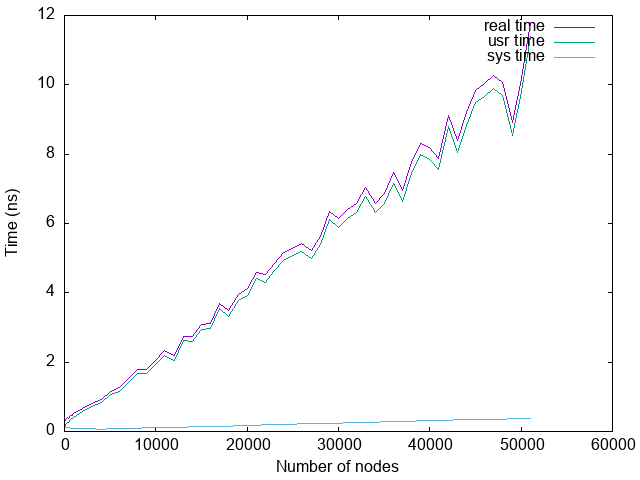
\includegraphics[width = 0.8\textwidth]{./images/average-prim-plot.png}
    \caption{Gráfica de tiempo del algoritmo de Prim para distintas cargas de trabajo.}
    \label{fig:prim-plot}
\end{figure}

\begin{figure}[H]
    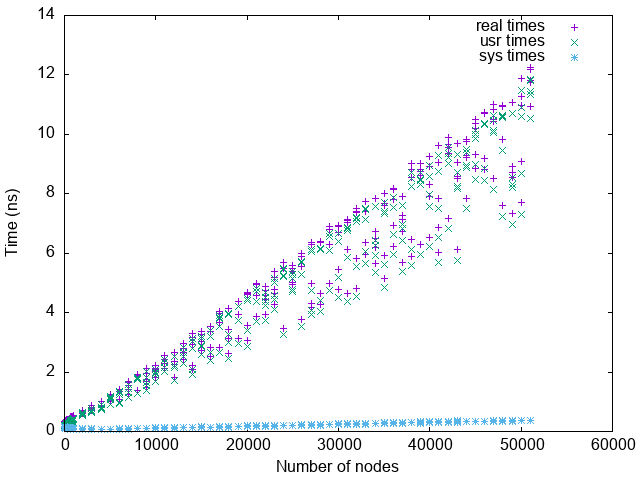
\includegraphics[width = 0.8\textwidth]{./images/prim-plot.png}
    \caption{Distribución de los tiempos observados en las distintas muestras del algoritmo de Prim para distintas cargas de trabajo.}
    \label{fig:prim-plot}
\end{figure}


\begin{figure}[H]
    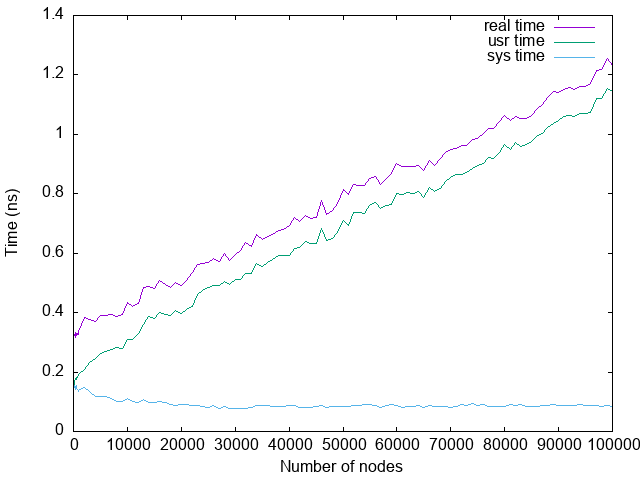
\includegraphics[width = 0.75\textwidth]{./images/average-decrease-key-plot.png}
    \caption{Gráfica de tiempo de Decrecer clave para varios tamaños de montículo.}
    \label{fig:decrease-key-plot}
\end{figure}

\begin{figure}[H]
    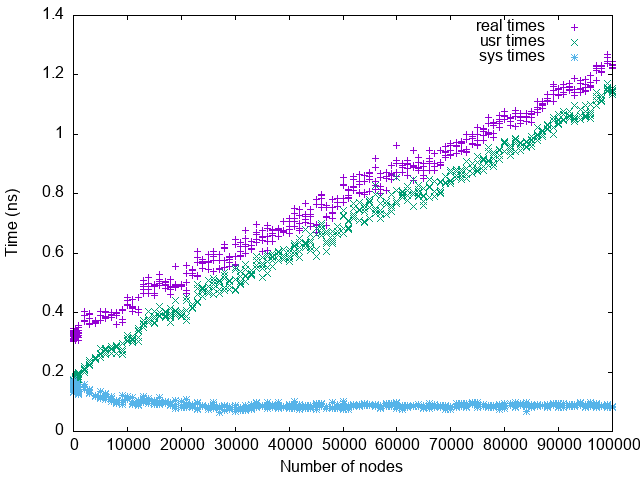
\includegraphics[width = 0.8\textwidth]{./images/decrease-key-plot.png}
    \caption{Distribución de los tiempos observados en las distintas muestras de Decrecer clave para distintas cargas de trabajo.}
    \label{fig:prim-plot}
\end{figure}




\end{document}
